\chapter{Rigging, skinning and animation}
\label{ch:animate}

\section{Skeletons and skins}
Bones are GameObjects with a Bone component under a root with an Armature, as Unity imports a character. A mesh
follows them through its \ui{Armature (Skin)} modifier: each vertex moves with the bones its vertex groups are named
after. Everything for characters is in the \textbf{Rigging} window: Skeleton, Skin, Transfer Weights, Vertex Groups,
Weight Paint, Auto-Rig, IK, Spring Bones, Anime Face Normals. Select a bone and drag its blue tail handle to aim and
stretch it; \key{Ctrl+E} extrudes a new bone from the tip; IK targets are boxes and poles diamonds, coloured by side
(left blue, right red); \ui{FK Controls} puts circles on bones to turn them by \cite{BlenderManual2026}.

\textbf{Automatic weights by inpainting} (Epic's method \cite{Abdrashitov2023Robust}): \ui{Bind: Automatic Weights}
gives each vertex that is clearly nearest one bone, and that the bone can see, to that bone; the rest get the
smoothest weights that agree with them, so nothing bleeds across a gap. \ui{Bind: Envelope} is the quick distance-only
binding. \ui{Transfer Weights} dresses a character: drag the rigged body onto \ui{From}; close matches copy the body's
weights and everything else is inpainted. \textbf{Weight Paint} fixes weights by hand (Add, Subtract, Draw, Blur, a
falloff, Mirror X; \key{Ctrl} or the pen's eraser subtracts).

\textbf{IK.} \ui{Add IK to Bone} on a shin or a forearm makes a target and a pole; \menu{GameObject > Rig > Humanoid /
Quadruped} makes a whole skeleton with IK; \ui{Auto IK} finds the limbs of an imported Mixamo, Unity or Rigify
skeleton by name; an IK constraint's Weight 0 is FK, and \ui{Switch to FK / IK} keeps the pose. \textbf{Auto-Rig with
markers} (Mixamo's way \cite{Mixamo2026}): select the mesh, \ui{Auto-Rig > Humanoid} or \ui{Quadruped}, click the
markers the diagram asks for (chin, wrists, elbows, knees, groin; Symmetry mirrors), then \ui{Build Rig}: the skeleton,
IK on every limb and the inpainted weights.

\begin{example}{rig a character in five minutes}
\begin{enumerate}
  \item Import or model the character standing in a T- or A-pose, facing +Z (Unity's forward).
  \item Select it; \ui{Rigging > Auto-Rig > Humanoid}. Click the chin, the left wrist, the left elbow, the left knee
    and the groin.
  \item \ui{Build Rig}. Select a hand's IK target and move it: the arm follows, the mesh with it.
  \item Fix any weight with Weight Paint (select the bone to paint its group).
\end{enumerate}
\end{example}

\textbf{Spring Bones} make hair, ears, tails and cloth strips swing after the animation (Stiffness, Damping, Gravity,
Radius and Collide against the body's capsules, Bend, Root To Tip, Separate, a Wind component), found automatically by
name on imported characters (Mixamo, VRM, Japanese rigs); \ui{Bake} writes the swing into a clip. \textbf{Soft tissue}
on one bone trails the body's acceleration and keeps its volume.

\section{The Animation window}
\menu{Window > Animation} is Unity's Animation window \cite{UnityManual2026}, a dopesheet laid out as Unity's: a
Summary row of every key, an object row per animated object, the property rows under it with their axes, each row a key
button and a value field you can type into.
\begin{enumerate}
  \item Select the object (a character's root, a door) and press \ui{Create}: it gets an \ui{Animation} component and a
    clip, \code{Assets/Animations/<name>.anim}.
  \item Turn on \ui{Record} (\key{Ctrl+Shift+K}). Move the playhead along the ruler and pose things with the gizmo or the
    Inspector: every change becomes a key at the playhead; right-click any Inspector field $>$ \ui{Insert Keyframe}
    (or \key{I} over it) keys a light's intensity, a material slot's colour, a modifier's amount, a blend shape's weight.
  \item Press play in the window (or turn on \ui{Preview} and scrub); in Play (\key{Ctrl+P}) the Animation component
    plays the clip: Loop, Once, Ping Pong or Clamp Forever, at any speed.
\end{enumerate}
\textbf{Keys:} click, \key{Shift}+click or a box to select; drag sideways to retime; \key{Delete}; \key{Ctrl+C} /
\key{Ctrl+V} at the playhead; \key{K} keys every track; comma and full stop step through the keys; right-click for
\ui{Auto} (Unity's Clamped Auto), \ui{Linear} or \ui{Constant}; \ui{Add Property} is a tree of the objects with their
components. \textbf{Curves}: the window's \ui{Curves} view shows how each value travels between keys; drag a key's
tangent handles (\ui{Free Smooth}), or right-click for \ui{Broken} (a bounce), \ui{Flat} (an ease) or \ui{Clamped Auto}.
A clip names objects by their path below the animated root, so it plays on any character with the same bone names;
IK runs after the clip, so animating the IK targets is enough for arms and legs. Animation on 2s or 3s holds frames
for the anime look.

\begin{figure}[H]
  \centering
  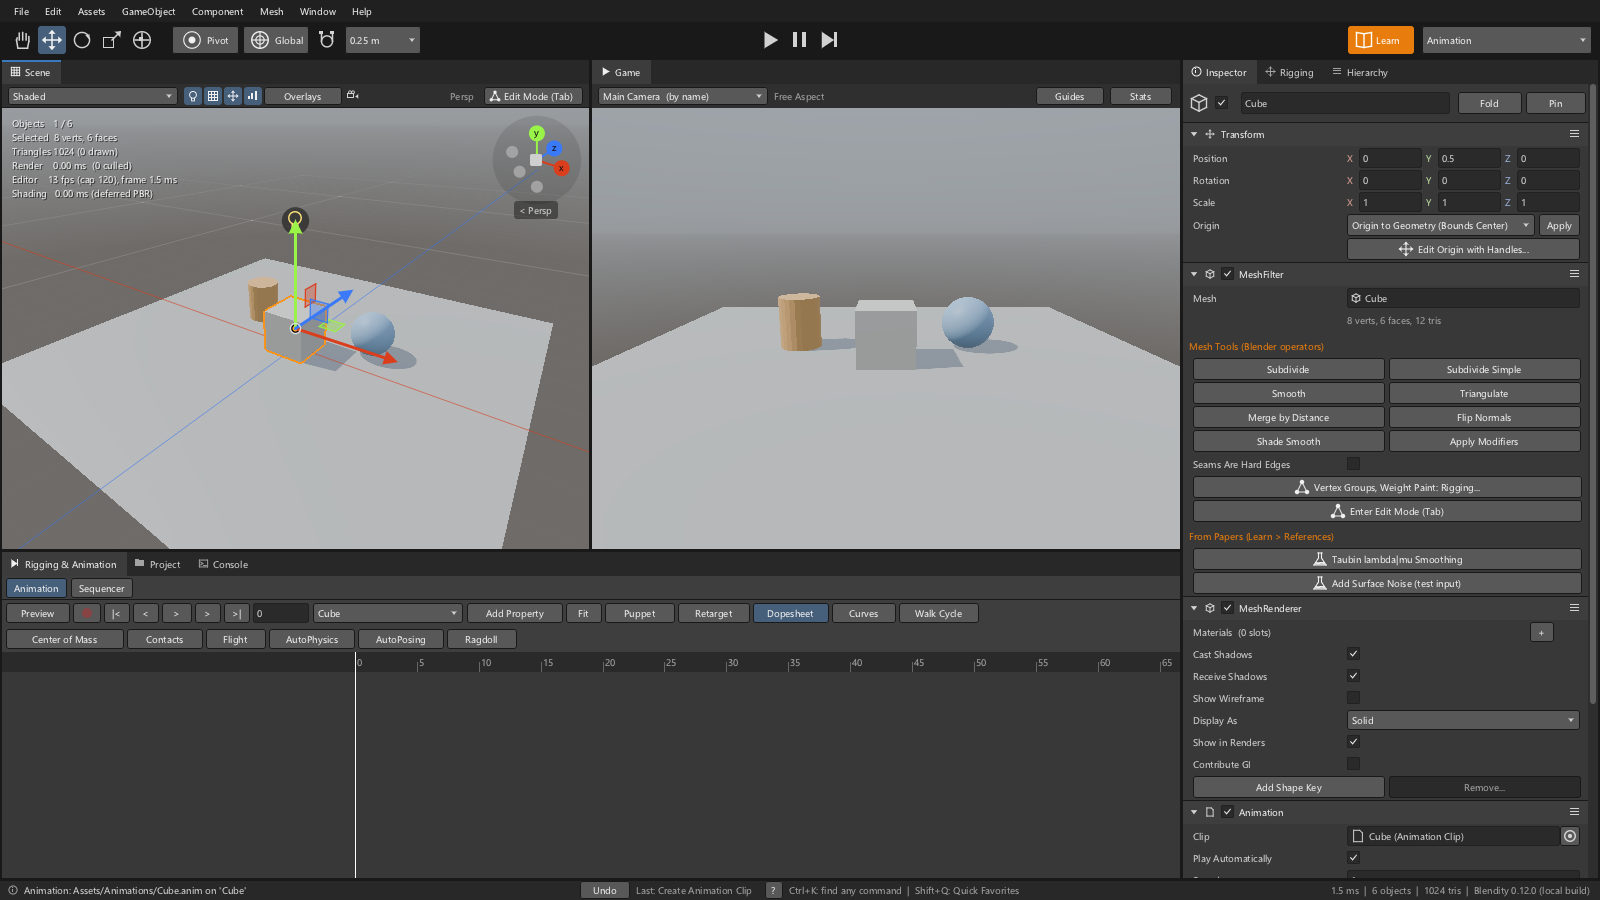
\includegraphics[width=\textwidth, alt={The Animation layout: the Scene view and the Game view above, the Animation window along the bottom with Preview, Record, the clip name, Add Property, Puppet, Retarget, Dopesheet and Curves, Walk Cycle and the physics tools, and the Rigging tab beside the Inspector.}]{layout-animation.png}
  \caption{The Animation layout: the Animation window along the bottom with Preview, Record, the clip, Add Property,
  Puppet, Retarget, Dopesheet / Curves, Walk Cycle and the physics tools; the Rigging tab beside the Inspector.}
\end{figure}

\begin{example}{a ball that bounces}
\begin{enumerate}
  \item Key the ball's Position y at 2 on frame 0, 0 on frame 15, 2 on frame 30.
  \item Curves view, click the Position.y track. Right-click the key on frame 15 $>$ \ui{Broken}.
  \item Drag its left handle steeply down and its right handle steeply up: the ball now hits the floor hard and leaves
    fast. Right-click the top keys $>$ \ui{Flat} for a hang at the top.
\end{enumerate}
\end{example}

\section{Puppet Posing and physics for animation}
Turn on \ui{AutoPosing} and the selected character's hands, feet, head and hips get controls in the Scene view: drag
one and the body follows, as motion capture would put a body there (a pose prior trained on the CMU database
\cite{Oreshkin2022Protores, CMUmocap2026}), the planted feet staying. Any humanoid rig works (Mixamo, the UE5 mannequin,
Character Creator, Daz, VRoid, Biped, Rigify; T or A pose). The \ui{Puppet} menu holds Reach, Motion Trails, Onion
Skin, the Zoetrope, Motion Check (sliding feet, pops and shaking, each with a Fix), the Smooth Brush and Lock in Place.
As in Cascadeur \cite{Cascadeur2026}: \ui{Center of Mass} weighs the body from its skin and follows it through a clip,
\ui{Contacts} are found from the motion and pinned, \ui{Flight} corrects a jump to a true parabola with its angular
momentum kept, \ui{AutoPhysics} makes the whole clip physically possible, take-offs and landings included, each shown
as a ghost before it is applied; \ui{Ragdoll} (Jolt) plays the clip with motors so hits and falls react. \ui{Walk Cycle}
makes walking and running cycles from the rig (feet never sliding, two legs or four), \ui{Footsteps} walks a character
along a curve on footprints you can move, \ui{Locomotion} walks and runs it live in Play. \ui{AI Inbetweening} (an
optional download) fills the motion between two keys in a style, shown as a ghost. Every assistant is a switch in
Preferences; hand animation never changes.

\section{Retargeting}
With a clip open on the rig it was made for, \ui{Retarget} lists the scene's other humanoid rigs; pick one and the clip
is remade for it by what each body part does (the 21 parts of the humanoid map found on any naming scheme), the hips'
moves scaled to its height and an A pose's arm drop reconciled with a T pose as Unity's Mecanim reads them
\cite{UnityHumanoidAvatars}; the new clip is saved beside the source's, set on the rig and opened. Fingers, the face
and IK are not carried.

\section{Sequencing clips}
\menu{Window > Sequencer} is a Premiere-style timeline for clips (instead of a state machine): press \ui{Create} and
drag \code{.anim} clips from the Project window onto its tracks; each bar is a clip and the object it plays on; drag
to move, its ends to trim; bars overlapping on one track crossfade; a higher track wins; \ui{Triggers} (a key, a clip,
blend seconds) jump to a clip in Play. The Sequencer also holds storyboard cards and camera cuts for animatics, WAV
sound mixed into Render Animation's video, footage, keyed opacity and transform, \ui{Add Edit} (\key{Alt+B}) and
\ui{Ripple Delete} (\key{Shift+Delete}).

\begin{fromnote}{Where it comes from}
Bones, skins and IK follow Blender's \cite{Blender2026, Welman1993Inverse}; the weights are Epic's inpainting
\cite{Abdrashitov2023Robust}; the marker auto-rig is Mixamo's workflow \cite{Mixamo2026}; the Animation window,
Record, the tangent modes, Humanoid retargeting and \code{.anim} clips are Unity's \cite{UnityManual2026,
UnityHumanoidAvatars}; the physics for animation follows Cascadeur's ideas \cite{Cascadeur2026}; the pose prior
follows ProtoRes \cite{Oreshkin2022Protores} on CMU data \cite{CMUmocap2026}; the spring chains follow Jakobsen and
the position-based solvers \cite{Jakobsen2001, Macklin2016}; the theory is in \cite{Gregory2018vol2} (animation,
physics). Learn: \emph{Modifiers vs Components} (vertex groups, weights, bones, IK, keyframes, curves, sequences),
\emph{Play Mode and the Game Loop}, \emph{Animating Any Property}.
\end{fromnote}
